\documentclass[border=10pt]{standalone}
\usepackage[svgnames]{xcolor}
\usepackage{amsmath}
\usepackage{pgfplots}
\pgfplotsset{compat=newest}
\usepackage[sfdefault]{FiraSans}
\usepackage{FiraMono}
\renewcommand*\familydefault{\sfdefault}
\begin{document}
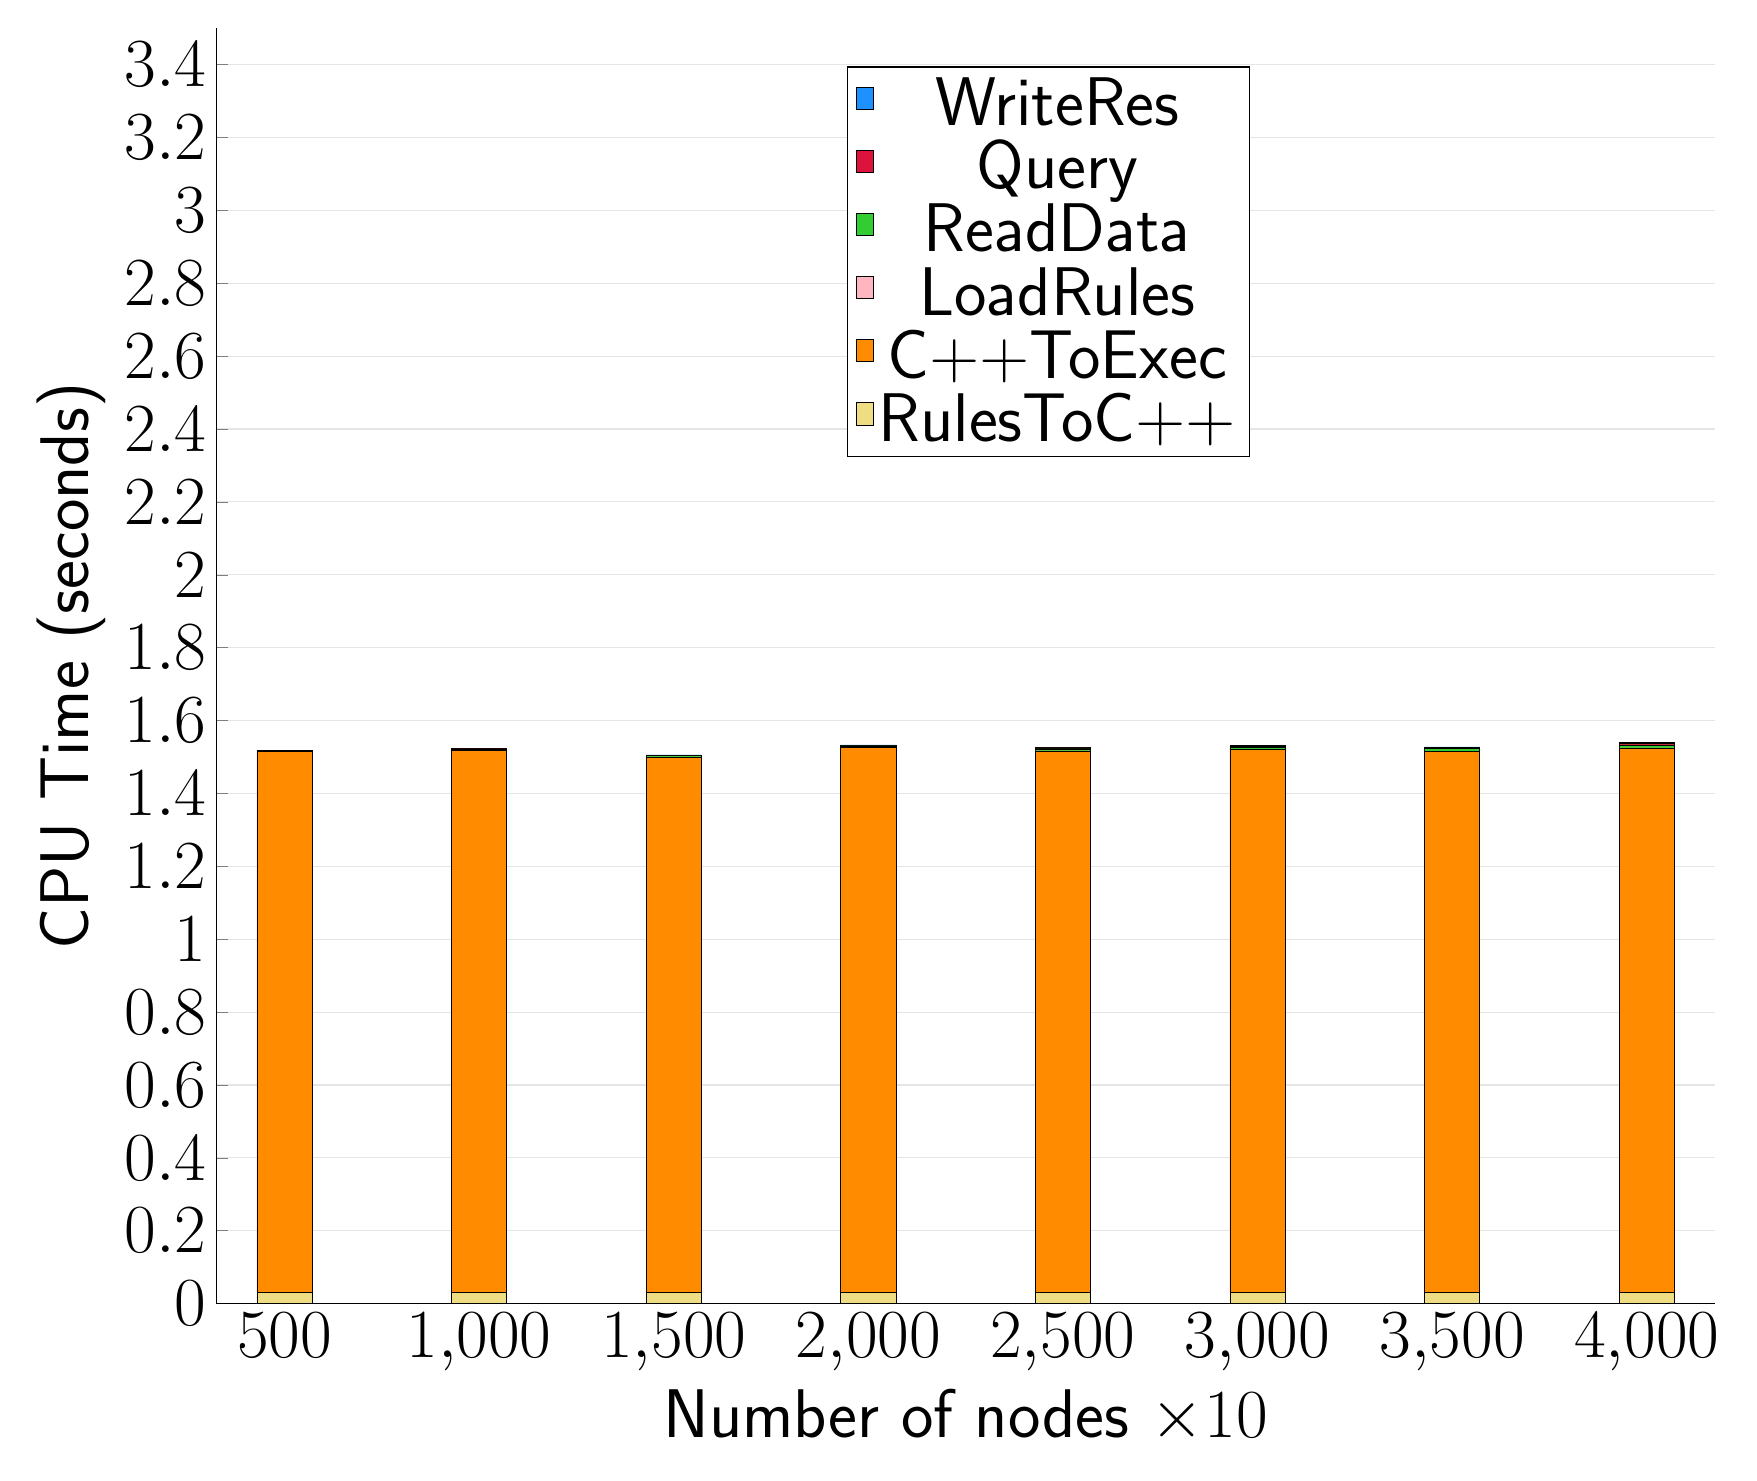
\begin{tikzpicture}
\begin{axis}[
   ybar stacked,
   width=1.7\textwidth,
   bar width=0.7cm,
   ymajorgrids, tick align=inside,
   major grid style={draw=gray!20},
   xtick=data,
   ymin=0, ymax=3.5,
   axis x line*=bottom,
   axis y line*=left,
   enlarge x limits=0.05,
   legend style={
       at={(0.69, 0.97)},
       anchor=north east,
       legend columns=1,
       font=\Huge,
   },
   ylabel={CPU Time (seconds)},
   xlabel={Number of nodes $\times 10$},
   label style={font=\Huge},
   tick label style={font=\Huge},
]
\addlegendimage{fill=DodgerBlue, draw=black, line width=0.2pt}
\addlegendentry{WriteRes}
\addlegendimage{fill=Crimson, draw=black, line width=0.2pt}
\addlegendentry{Query}
\addlegendimage{fill=LimeGreen, draw=black, line width=0.2pt}
\addlegendentry{ReadData}
\addlegendimage{fill=LightPink, draw=black, line width=0.2pt}
\addlegendentry{LoadRules}
\addlegendimage{fill=DarkOrange, draw=black, line width=0.2pt}
\addlegendentry{C++ToExec}
\addlegendimage{fill=LightGoldenrod, draw=black, line width=0.2pt}
\addlegendentry{RulesToC++}
\addplot +[fill=LightGoldenrod, draw=black, line width=0.2pt] coordinates {
(500, 0.030000000000000006)
(1000, 0.030000000000000006)
(1500, 0.030000000000000006)
(2000, 0.030000000000000006)
(2500, 0.031000000000000007)
(3000, 0.030000000000000006)
(3500, 0.030000000000000006)
(4000, 0.030000000000000006)
};
\addplot +[fill=DarkOrange, draw=black, line width=0.2pt] coordinates {
(500, 1.486)
(1000, 1.4890000000000003)
(1500, 1.4699999999999998)
(2000, 1.496)
(2500, 1.4860000000000002)
(3000, 1.491)
(3500, 1.485)
(4000, 1.4949999999999999)
};
\addplot +[fill=LightPink, draw=black, line width=0.2pt] coordinates {
(500, 7.41e-05)
(1000, 0.000101)
(1500, 0.00011060000000000002)
(2000, 0.0001104)
(2500, 8.319999999999999e-05)
(3000, 6.860000000000001e-05)
(3500, 0.0001209)
(4000, 0.00011)
};
\addplot +[fill=LimeGreen, draw=black, line width=0.2pt] coordinates {
(500, 0.001131)
(1000, 0.0024238)
(1500, 0.0034053)
(2000, 0.0044318)
(2500, 0.0052959)
(3000, 0.0060579)
(3500, 0.0077147)
(4000, 0.008284999999999999)
};
\addplot +[fill=Crimson, draw=black, line width=0.2pt] coordinates {
(500, 0.0004376999999999999)
(1000, 0.0010538)
(1500, 0.0015428)
(2000, 0.0019511)
(2500, 0.0024622000000000003)
(3000, 0.0028393000000000003)
(3500, 0.003624)
(4000, 0.0041826)
};
\addplot +[fill=DodgerBlue, draw=black, line width=0.2pt] coordinates {
(500, 0.00037520000000000007)
(1000, 0.0006571000000000001)
(1500, 0.0008213)
(2000, 0.0010425)
(2500, 0.0011975000000000002)
(3000, 0.001309)
(3500, 0.0016054000000000003)
(4000, 0.0016965)
};
\end{axis}
\end{tikzpicture}

\end{document}
